
\begin{definition}
A \term{linear transformation} (also known as a \term{linear map})
is a map between vector spaces that preserves the vector space operations.
More precisely, if \(V\) and $W$ are vector spaces, a map
\(T:V\rightarrow W\) is called a linear transformation if
\begin{enumerate}
\item \(T(\vec{v}+\vec{w}) = T(\vec{v})+T(\vec{w})\)
      for any \(\vec{v},\vec{w} \in V\).
\item \(T(c\vec{v}) = cT(\vec{v})\)
      for any \(c \in \IR,\vec{v} \in V\).
\end{enumerate}
In other words, a map is linear when vector space operations
can be applied before or after the transformation without affecting the result.
\end{definition}

\begin{definition}
Given a linear transformation \(T:V\to W\),
\(V\) is called the \term{domain} of \(T\) and
\(W\) is called the \term{co-domain} of \(T\).

\begin{center}
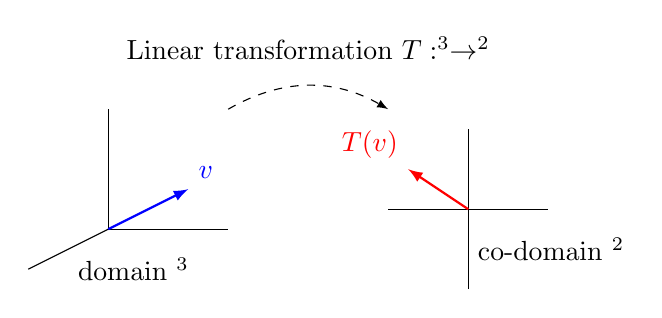
\begin{tikzpicture}[x=0.2in,y=0.2in]
  \begin{scope}[shift={(0,0)}]
    \draw (0,0) -- (3,0);
    \draw (0,0) -- (0,3);
    \draw (0,0) -- (-2,-1);
    \draw[thick,-latex,blue] (0,0) -- (2,1)
          node[anchor=south west] {\(\vect v\)};
    \node[anchor=west] at (-1,-1) {domain \(\IR^3\)};
  \end{scope}
  \draw[dashed,-latex] (3,3) to [bend left=30] (7,3);
  \node[anchor=south] at (5,4) {Linear transformation \(T:\IR^3\to\IR^2\)};
  \begin{scope}[shift={(9,0.5)}]
    \draw (-2,0) -- (2,0);
    \draw (0,-2) -- (0,2);
    \draw[thick,-latex,red] (0,0) -- (-1.5,1)
          node[anchor=south east] {\(T(\vect v)\)};
    \node[anchor=west] at (0,-1) {co-domain \(\IR^2\)};
  \end{scope}
\end{tikzpicture}
\end{center}
\end{definition}

\begin{example}
Let \(T : \IR^3 \rightarrow \IR^2\) be given by
\[
  T\left(\begin{bmatrix} x \\ y \\ z \end{bmatrix} \right)
=
  \begin{bmatrix} x-z \\ 3y \end{bmatrix}
\]

To show that \(T\) is linear, we must verify...
\[
  T\left(
    \begin{bmatrix} x \\ y \\ z \end{bmatrix} +
    \begin{bmatrix} u \\ v \\ w \end{bmatrix}
  \right)
=
  T\left(
    \begin{bmatrix} x+u \\ y+v \\ z+w \end{bmatrix}
  \right) =
  \begin{bmatrix} (x+u)-(z+w) \\ 3(y+v) \end{bmatrix}
\]
\[
  T\left(
    \begin{bmatrix} x \\ y \\ z \end{bmatrix}
  \right) + T\left(
    \begin{bmatrix} u \\ v \\ w \end{bmatrix}
  \right)
=
  \begin{bmatrix} x-z \\ 3y \end{bmatrix} +
  \begin{bmatrix} u-w \\ 3v \end{bmatrix}=
  \begin{bmatrix} (x+u)-(z+w) \\ 3(y+v) \end{bmatrix}
\]
And also...
\[
  T\left(c\begin{bmatrix} x \\ y \\ z \end{bmatrix} \right)
=
  T\left(\begin{bmatrix} cx \\ cy \\ cz \end{bmatrix} \right)
=
  \begin{bmatrix} cx-cz \\ 3cy \end{bmatrix}
\text{ and }
  cT\left(\begin{bmatrix} x \\ y \\ z \end{bmatrix} \right)
=
  c\begin{bmatrix} x-z \\ 3y \end{bmatrix}
=
  \begin{bmatrix} cx-cz \\ 3cy \end{bmatrix}
\]

Therefore \(T\) is a linear transformation.
\end{example}

\begin{example}
Let \(T : \IR^2 \rightarrow \IR^4\) be given by
\[
  T\left(\begin{bmatrix} x \\ y \end{bmatrix} \right)
=
  \begin{bmatrix} x+y \\ x^2 \\ y+3 \\ y-2^x \end{bmatrix}
\]

To show that \(T\) is not linear, we only need to find one
counterexample.
\[
  T\left(
    \begin{bmatrix} 0 \\ 1 \end{bmatrix} +
    \begin{bmatrix} 2 \\ 3 \end{bmatrix}
  \right)
=
  T\left(
    \begin{bmatrix} 2 \\ 4 \end{bmatrix}
  \right) =
  \begin{bmatrix} 6 \\ 4 \\ 7 \\ 0 \end{bmatrix}
\]
\[
  T\left(
    \begin{bmatrix} 0 \\ 1 \end{bmatrix}
  \right) + T\left(
    \begin{bmatrix} 2 \\ 3\end{bmatrix}
  \right)
=
  \begin{bmatrix} 1 \\ 0 \\ 4 \\ -1 \end{bmatrix} +
  \begin{bmatrix} 5 \\ 4 \\ 6 \\ -5 \end{bmatrix}
=
  \begin{bmatrix} 6 \\ 4 \\ 10 \\ -6 \end{bmatrix}
\]

Since the resulting vectors are different,
\(T\) is not a linear transformation.
\end{example}

\begin{fact}
A map between Euclidean spaces \(T:\IR^n\to\IR^m\) is linear
exactly when every component of the output is a linear combination
of the variables of \(\IR^n\).

\vspace{1em}

For example, the following map is definitely linear
because \(x-z\) and \(3y\) are linear combinations of \(x,y,z\):
\[
  T\left(\begin{bmatrix} x \\ y \\ z \end{bmatrix} \right)
=
  \begin{bmatrix} x-z \\ 3y \end{bmatrix}
=
  \begin{bmatrix} 1x+0y-1z \\ 0x+3y+0z \end{bmatrix}
\]

But this map is not linear because \(x^2\), \(y+3\), and \(y-2^x\)
are not linear combinations (even though \(x+y\) is):
\[
  T\left(\begin{bmatrix} x \\ y \end{bmatrix} \right)
=
  \begin{bmatrix} x+y \\ x^2 \\ y+3 \\ y-2^x \end{bmatrix}
\]
\end{fact}

\begin{activity}{5}
  Recall the following rules from calculus, where \(D:\P\to\P\)
  is the derivative map defined by \(D(f(x))=f'(x)\) for each
  polynomial \(f\).
  \[
    D(f+g)=f'(x)+g'(x)
  \]
  \[
    D(cf(x))=cf'(x)
  \]
  What can we conclude from these rules?
  \begin{enumerate}[a)]
    \item \(\P\) is not a vector space
    \item \(D\) is a linear map
    \item \(D\) is not a linear map
  \end{enumerate}
\end{activity}


\begin{activity}{10}
Let the polynomial maps \(S: \P^4 \rightarrow \P^3\)
and \(T: \P^4 \rightarrow \P^3\) be defined by

\[S(f(x)) = 2f'(x)-f''(x) \hspace{3em} T(f(x)) = f'(x)+x^3\]

Compute \(S(x^4+x)\), \(S(x^4)+S(x)\), \(T(x^4+x)\), and \(T(x^4)+T(x)\).
Which of these maps is definitely not linear?
\end{activity}


\begin{fact}
If \(L:V\to W\) is linear, then \(L(\vec z)=L(0\vec v)=0L(\vec v)=\vec z\)
where \(\vec z\) is the additive identity of the vector spaces \(V,W\).

\vspace{1em}

Put another way, an easy way to prove that a map like
\(T(f(x)) = f'(x)+x^3\) can't be linear is because
\[T(0)=\frac{d}{dx}[0]+x^3=0+x^3=x^3\not=0.\]
\end{fact}

\begin{observation}
Showing \(L:V\to W\) is not a linear transformation can be done by finding an example
for any one of the following.

\begin{itemize}
\item Show \(L(\vec z)\not=\vec z\) (where \(\vec z\) is the additive identity of \(L\) and \(W\)).
\item Find \(\vec v,\vec w\in V\) such that \(L(\vec v+\vec w)\not=L(\vec v)+L(\vec w)\).
\item Find \(\vec v\in V\) and \(c\in \IR\) such that \(L(c\vec v)\not=cL(\vec v)\).
\end{itemize}

Otherwise, \(L\) can be shown to be linear by proving the following in general.

\begin{itemize}
\item For all \(\vec v,\vec w\in V\), \(L(\vec v+\vec w)=L(\vec v)+L(\vec w)\).
\item For all \(\vec v\in V\) and \(c\in \IR\), \(L(c\vec v)=cL(\vec v)\).
\end{itemize}

Note the similarities between this process and showing that a subset of a vector
space is/isn't a subspace. 
\end{observation}

\begin{activity}{15}
Continue to consider \(S: \P^4 \rightarrow \P^3\) defined by

\[S(f(x)) = 2f'(x)-f''(x)\]

\begin{subactivity}
  Verify that
  \[S(f(x)+g(x))=2f'(x)+2g'(x)-f''(x)-g''(x)\]
  is equal to \(S(f(x))+S(g(x))\) for all polynomials \(f,g\).
\end{subactivity}
\begin{subactivity}
  Verify that \(S(cf(x))\) is equal to \(cS(f(x))\) for all real numbers \(c\)
  and polynomials \(f\). 
\end{subactivity}
\begin{subactivity}
  Is \(S\) linear?
\end{subactivity}
\end{activity}


\begin{activity}{20}
Let the polynomial maps \(S: \P \rightarrow \P\)
and \(T: \P \rightarrow \P\) be defined by

\[S(f(x)) = (f(x))^2 \hspace{3em} T(f(x)) = 3xf(x^2)\]

\begin{subactivity}
Note that \(S(0)=0\) and \(T(0)=0\). So instead,
show that \(S(x+1)\not= S(x)+S(1)\) to verify that \(S\) is not linear.
\end{subactivity}
\begin{subactivity}
Prove that \(T\) is linear by verifying that \(T(f(x)+g(x))=T(f(x))+T(g(x))\)
and \(T(cf(x))=cT(f(x))\).
\end{subactivity}
\end{activity}


\begin{remark}
Recall that a linear map \(T:V\rightarrow W\)
satisfies
\begin{enumerate}
\item \(T(\vec{v}+\vec{w}) = T(\vec{v})+T(\vec{w})\)
      for any \(\vec{v},\vec{w} \in V\).
\item \(T(c\vec{v}) = cT(\vec{v})\)
      for any \(c \in \IR,\vec{v} \in V\).
\end{enumerate}
In other words, a map is linear when vector space operations
can be applied before or after the transformation without affecting the result.
\end{remark}

\begin{activity}{5}
Suppose \(T: \IR^3 \rightarrow \IR^2\) is a linear map, and you know
\(
  T\left(\begin{bmatrix} 1 \\ 0 \\ 0 \end{bmatrix} \right)
=
  \begin{bmatrix} 2 \\ 1 \end{bmatrix}
\)
and
\(
  T\left(\begin{bmatrix} 0 \\ 0 \\ 1 \end{bmatrix} \right)
=
  \begin{bmatrix} -3 \\ 2 \end{bmatrix}
\).
Compute \(T\left(\begin{bmatrix} 3 \\ 0 \\ 0 \end{bmatrix}\right)\).
\begin{multicols}{2}
\begin{enumerate}[(a)]
\item \(\begin{bmatrix} 6 \\ 3\end{bmatrix}\)
\item \(\begin{bmatrix} -9 \\ 6 \end{bmatrix}\)
\item \(\begin{bmatrix} -4 \\ -2 \end{bmatrix}\)
\item \(\begin{bmatrix} 6 \\ -4 \end{bmatrix}\)
\end{enumerate}
\end{multicols}
\end{activity}

\begin{activity}{5}
Suppose \(T: \IR^3 \rightarrow \IR^2\) is a linear map, and you know
\(
  T\left(\begin{bmatrix} 1 \\ 0 \\ 0 \end{bmatrix} \right)
=
  \begin{bmatrix} 2 \\ 1 \end{bmatrix}
\)
and
\(
  T\left(\begin{bmatrix} 0 \\ 0 \\ 1 \end{bmatrix} \right)
=
  \begin{bmatrix} -3 \\ 2 \end{bmatrix}
\).
Compute \(T\left(\begin{bmatrix} 1 \\ 0 \\ 1 \end{bmatrix}\right)\).
\begin{multicols}{2}
\begin{enumerate}[(a)]
\item \(\begin{bmatrix} 2 \\ 1\end{bmatrix}\)
\item \(\begin{bmatrix} 3 \\ -1 \end{bmatrix}\)
\item \(\begin{bmatrix} -1 \\ 3 \end{bmatrix}\)
\item \(\begin{bmatrix} 5 \\ -8 \end{bmatrix}\)
\end{enumerate}
\end{multicols}
\end{activity}

\begin{activity}{5}
Suppose \(T: \IR^3 \rightarrow \IR^2\) is a linear map, and you know
\(
  T\left(\begin{bmatrix} 1 \\ 0 \\ 0 \end{bmatrix} \right)
=
  \begin{bmatrix} 2 \\ 1 \end{bmatrix}
\)
and
\(
  T\left(\begin{bmatrix} 0 \\ 0 \\ 1 \end{bmatrix} \right)
=
  \begin{bmatrix} -3 \\ 2 \end{bmatrix}
\).
Compute \(T\left(\begin{bmatrix} -2 \\ 0 \\ -3 \end{bmatrix}\right)\).
\begin{multicols}{2}
\begin{enumerate}[(a)]
\item \(\begin{bmatrix} 2 \\ 1\end{bmatrix}\)
\item \(\begin{bmatrix} 3 \\ -1 \end{bmatrix}\)
\item \(\begin{bmatrix} -1 \\ 3 \end{bmatrix}\)
\item \(\begin{bmatrix} 5 \\ -8 \end{bmatrix}\)
\end{enumerate}
\end{multicols}
\end{activity}

\begin{activity}{5}
Suppose \(T: \IR^3 \rightarrow \IR^2\) is a linear map, and you know
\(
  T\left(\begin{bmatrix} 1 \\ 0 \\ 0 \end{bmatrix} \right)
=
  \begin{bmatrix} 2 \\ 1 \end{bmatrix}
\)
and
\(
  T\left(\begin{bmatrix} 0 \\ 0 \\ 1 \end{bmatrix} \right)
=
  \begin{bmatrix} -3 \\ 2 \end{bmatrix}
\).

What piece of information would help you compute \(T\left(\begin{bmatrix}0\\4\\-1\end{bmatrix}\right)\)?
\begin{multicols}{2}
\begin{enumerate}[(a)]
\item The value of \(T\left(\begin{bmatrix} 0\\-4\\0\end{bmatrix}\right)\).
\item The value of \(T\left(\begin{bmatrix} 0\\1\\0\end{bmatrix}\right)\).
\item The value of \(T\left(\begin{bmatrix} 1\\1\\1\end{bmatrix}\right)\).
\item Any of the above.
\end{enumerate}
\end{multicols}
\end{activity}

\begin{fact}
Consider any basis \(\{\vec b_1,\dots,\vec b_n\}\) for $V$.  Since every
vector \(\vec v\) can be written as a linear combination of
basis vectors, \(x_1\vec b_1+\dots+ x_n\vec b_n\), we may compute
\(T(\vec v)\) as follows:

\[
  T(\vec v)=T(x_1\vec b_1+\dots+ x_n\vec b_n)=
  x_1T(\vec b_1)+\dots+x_nT(\vec b_n)
.\]

Therefore any linear transformation \(T:V \rightarrow W\) can be defined
by just describing the values of \(T(\vec b_i)\).

Put another way, the images of the basis vectors \term{determine} the transformation \(T\).
\end{fact}

\begin{definition}
Since linear transformation \(T:\IR^n\to\IR^m\) is determined by
the standard basis \(\{\vec e_1,\dots,\vec e_n\}\), it's convenient to
store this information in the \(m\times n\) \term{standard matrix}
\([T(\vec e_1) \,\cdots\, T(\vec e_n)]\).

\vspace{1em}

For example,
let \(T: \IR^3 \rightarrow \IR^2\) be the linear map determined by
the following values for \(T\) applied to the standard basis of \(\IR^3\).

\[\scriptsize
  T\left(\vec e_1 \right)
=
  T\left(\begin{bmatrix} 1 \\ 0 \\ 0 \end{bmatrix} \right)
=
  \begin{bmatrix} 3 \\ 2\end{bmatrix}
\hspace{2em}
  T\left(\vec e_2 \right)
=
  T\left(\begin{bmatrix} 0 \\ 1 \\ 0 \end{bmatrix} \right)
=
  \begin{bmatrix} -1 \\ 4\end{bmatrix}
\hspace{2em}
  T\left(\vec e_3 \right)
=
  T\left(\begin{bmatrix} 0 \\ 0 \\ 1 \end{bmatrix} \right)
=
  \begin{bmatrix} 5 \\ 0\end{bmatrix}
\]

Then the standard matrix corresponding to \(T\) is
\[
  \begin{bmatrix}T(\vec e_1) & T(\vec e_2) & T(\vec e_3)\end{bmatrix}
=
  \begin{bmatrix}3 & -1 & 5 \\ 2 & 4 & 0 \end{bmatrix}
.\]
\end{definition}

\begin{activity}{3}
  Let $T: \IR^4 \rightarrow \IR^3$ be the linear transformation given by
  \[
    T\left(\vec e_1 \right)
  =
    \begin{bmatrix} 0 \\ 3 \\ -2\end{bmatrix}
  \hspace{2em}
    T\left(\vec e_2 \right)
  =
    \begin{bmatrix} -3 \\ 0 \\ 1\end{bmatrix}
  \hspace{2em}
    T\left(\vec e_3 \right)
  =
    \begin{bmatrix} 4 \\ -2 \\ 1\end{bmatrix}
  \hspace{2em}
    T\left(\vec e_4 \right)
  =
    \begin{bmatrix} 2 \\ 0 \\ 0\end{bmatrix}
  \]
Write the standard matrix \([T(\vec e_1) \,\cdots\, T(\vec e_n)]\) for \(T\).
\end{activity}

\begin{activity}{5}
  Let \(T: \IR^3 \rightarrow \IR^2\) be the linear transformation given by
\[T\left(\begin{bmatrix} x\\ y \\ z \end{bmatrix} \right) = \begin{bmatrix} x+3z \\ 2x-y-4z \end{bmatrix}\]
\begin{subactivity}
Compute \(T(\vec e_1)\), \(T(\vec e_2)\), and \(T(\vec e_3)\).
\end{subactivity}
\begin{subactivity}
Find the standard matrix for \(T\).
\end{subactivity}
\end{activity}

\begin{fact}
  Because every linear map \(T:\IR^m\to\IR^n\) has a linear combination
  of the variables in each component, and thus
  \(T(\vec e_i)\) yields exactly the coefficients of \(x_i\),
  the standard matrix for \(T\) is simply an ordered list of
  the coefficients of the \(x_i\):
  \[
    T\left(\begin{bmatrix}x\\y\\z\\w\end{bmatrix}\right)
      =
    \begin{bmatrix}
      ax+by+cz+dw \\
      ex+fy+gz+hw
    \end{bmatrix}
  \hspace{2em}
    A
      =
    \begin{bmatrix}
      a & b & c & d \\
      e & f & g & h
    \end{bmatrix}
  \]
\end{fact}

\begin{activity}{5}
  Let $T: \IR^3 \rightarrow \IR^3$ be the linear transformation given by the standard matrix
  \[
    \begin{bmatrix} 3  & -2 & -1  \\ 4 & 5 & 2 \\ 0 & -2 & 1 \end{bmatrix}
  .\]

\begin{subactivity}
Compute $T\left(\begin{bmatrix} x\\ y \\ z \end{bmatrix} \right) $.
\end{subactivity}
\begin{subactivity}
Compute $T\left(\begin{bmatrix} 1\\ 2 \\ 3 \end{bmatrix} \right) $.
\end{subactivity}
\end{activity}

\begin{fact}
  To quickly compute \(T(\vec v)\) from its standard matrix \(A\),
  multiply and add the entries of each row of \(A\) with the vector \(\vec v\).
  For example, if \(T\) has the standard matrix
  \[
    A = \begin{bmatrix} 1 & 2 & 3 \\ 0 & 1 & -2 \\ 2 & -1 & 0 \end{bmatrix}
  \]
  then for \(\vec v=\begin{bmatrix}x\\y\\z\end{bmatrix}\) we will write
  \[
    T(\vec v)
      =
    A\vec v
      =
    \begin{bmatrix} 1 & 2 & 3 \\ 0 & 1 & -2 \\ 2 & -1 & 0 \end{bmatrix}
    \begin{bmatrix}x\\y\\z\end{bmatrix}
      =
    \begin{bmatrix}
      1x+2y+3z\\
      0x+1y-2z\\
      2x-1y+0z
    \end{bmatrix}
  \]
  and for \(\vec v=\begin{bmatrix}3\\0\\-2\end{bmatrix}\) we will write
  \[
    T(\vec v)
      =
    A\vec v
      =
    \begin{bmatrix} 1 & 2 & 3 \\ 0 & 1 & -2 \\ 2 & -1 & 0 \end{bmatrix}
    \begin{bmatrix}3\\0\\-2\end{bmatrix}
      =
    \begin{bmatrix}
      1(3)+2(0)+3(-2)\\
      0(3)+1(0)-2(-2)\\
      2(3)-1(0)+0(-2)
    \end{bmatrix}
      =
    \begin{bmatrix}
      -3\\
      4\\
      6
    \end{bmatrix}
  .\]
\end{fact}

\begin{activity}{15}
  Compute the following linear transformations of vectors given their
  standard matrices.
  \[
    T_1\left(\begin{bmatrix}1\\2\end{bmatrix}\right)
    \text{ for the standard matrix }
    A_1=\begin{bmatrix}4&3\\0&-1\\1&1\\3&0\end{bmatrix}
  \]
  \[
    T_2\left(\begin{bmatrix}1\\1\\0\\-3\end{bmatrix}\right)
    \text{ for the standard matrix }
    A_2=\begin{bmatrix}4&3&0&-1\\1&1&3&0\end{bmatrix}
  \]
  \[
    T_3\left(\begin{bmatrix}0\\-2\\0\end{bmatrix}\right)
    \text{ for the standard matrix }
    A_3=\begin{bmatrix}4&3&0\\0&-1&3\\5&1&1\\3&0&0\end{bmatrix}
  \]
\end{activity}


\begin{definition}
Let $T: V \rightarrow W$ be a linear transformation.  The \term{kernel} of $T$
is an important subspace of \(V\) defined by
\[
\ker T = \left\{ \vec{v} \in V\ \big|\ T(\vec{v})=\vec{z}\right\}
\]

\begin{center}
  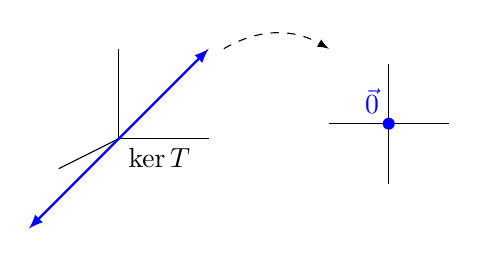
\begin{tikzpicture}[x=0.15in,y=0.15in]
    \begin{scope}[shift={(0,0)}]
      \draw (0,0) node[anchor=north west] {\(\ker T\)} -- (3,0);
      \draw (0,0) -- (0,3);
      \draw (0,0)  -- (-2,-1);
      \draw[thick,latex-latex,blue] (-3,-3) -- (3,3);
    \end{scope}
    \draw[dashed,-latex] (3.5,3) to [bend left=30] (7,3);
    \begin{scope}[shift={(9,0.5)}]
      \draw (-2,0) -- (2,0);
      \draw (0,-2) -- (0,2);
      \fill[blue] (0,0) circle (0.2)
            node[anchor=south east] {\(\vec{0}\)};
    \end{scope}
  \end{tikzpicture}
\end{center}
\end{definition}

\begin{activity}{5}
Let $T: \IR^2 \rightarrow \IR^3$ be given by
\[
  T\left(\begin{bmatrix}x \\ y \end{bmatrix} \right)
    =
  \begin{bmatrix} x \\ y \\ 0 \end{bmatrix}
    \hspace{3em}
    \text{with standard matrix }
  \begin{bmatrix} 1 & 0 \\ 0 & 1 \\ 0 & 0 \end{bmatrix}
\]
Which of these subspaces of \(\IR^2\) describes \(\ker T\),
the set of all vectors that transform into \(\vec 0\)?
\begin{enumerate}[a)]
\item \(\setBuilder{\begin{bmatrix}a \\ a\end{bmatrix}}{a\in\IR}\)
\item \(\setList{\begin{bmatrix}0\\0\end{bmatrix}}\)
\item \(\IR^2=\setBuilder{\begin{bmatrix}x \\ y\end{bmatrix}}{x,y\in\IR}\)
\end{enumerate}
\end{activity}

\begin{activity}{5}
Let $T: \IR^3 \rightarrow \IR^2$ be given by
\[
  T\left(\begin{bmatrix}x \\ y\\z \end{bmatrix} \right)
    =
  \begin{bmatrix} x \\ y \end{bmatrix}
    \hspace{3em}
    \text{with standard matrix }
  \begin{bmatrix} 1 & 0 & 0 \\ 0 & 1 & 0 \end{bmatrix}
\]
Which of these subspaces of \(\IR^3\) describes \(\ker T\),
the set of all vectors that transform into \(\vec 0\)?
\begin{multicols}{2}
\begin{enumerate}[a)]
\item \(\setBuilder{\begin{bmatrix}0 \\ 0\\ a\end{bmatrix}}{a\in\IR}\)
\item \(\setBuilder{\begin{bmatrix}a \\ a\\ 0\end{bmatrix}}{a\in\IR}\)
\item \(\setList{\begin{bmatrix}0\\0\\0\end{bmatrix}}\)
\item \(\IR^3=\setBuilder{\begin{bmatrix}x \\ y\\z\end{bmatrix}}{x,y,z\in\IR}\)
\end{enumerate}
\end{multicols}
\end{activity}

\begin{activity}{10}
Let $T: \IR^3 \rightarrow \IR^2$ be the linear transformation given by the
standard matrix
\[A=\begin{bmatrix} 3 & 4 & -1 \\ 1 & 2 & 1 \end{bmatrix}.\]
\begin{subactivity}
Set
\(
  T\left(\begin{bmatrix}x\\y\\z\end{bmatrix}\right)
    =
  \begin{bmatrix}
    \unknown+\unknown+\unknown \\
    \unknown+\unknown+\unknown
  \end{bmatrix}
    =
  \begin{bmatrix}0\\0\end{bmatrix}
\) to find a linear system of equations whose solution set is the kernel.
\end{subactivity}
\begin{subactivity}
Use $\RREF(A)$ to solve this homogeneous system of equations and find a basis
for the kernel of \(T\).
\end{subactivity}
\end{activity}


\begin{definition}
Let $T: V \rightarrow W$ be a linear transformation.
The \term{image} of $T$ is an important subspace of \(W\) defined by
\[
\Im T = \left\{ \vec{w} \in W\ \big|\ \text{there is some }\vec v\in V \text{ with } T(\vec{v})=\vec{w}\right\}
\]
In the examples below, the left example's image is all of \(\IR^2\), but the
right example's image is a planar subspace of \(\IR^3\).
\begin{center}
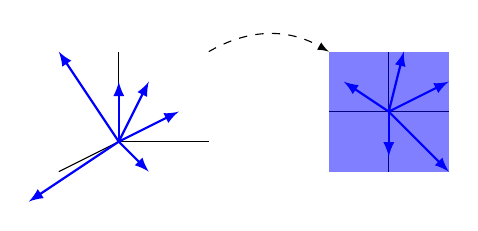
\begin{tikzpicture}[x=0.15in,y=0.15in]
  \begin{scope}[shift={(0,0)}]
    \draw (0,0) -- (3,0);
    \draw (0,0) -- (0,3);
    \draw (0,0) -- (-2,-1);
    \draw[thick,-latex,blue] (0,0) -- (2,1);
    \draw[thick,-latex,blue] (0,0) -- (1,2);
    \draw[thick,-latex,blue] (0,0) -- (0,2);
    \draw[thick,-latex,blue] (0,0) -- (1,-1);
    \draw[thick,-latex,blue] (0,0) -- (-2,3);
    \draw[thick,-latex,blue] (0,0) -- (-3,-2);
  \end{scope}
  \draw[dashed,-latex] (3,3) to [bend left=30] (7,3);
  \begin{scope}[shift={(9,1)}]
    \draw (-2,0) -- (2,0);
    \draw (0,-2) -- (0,2);
    \draw[thick,-latex,blue] (0,0) -- (0.5,2);
    \draw[thick,-latex,blue] (0,0) -- (2,1);
    \draw[thick,-latex,blue] (0,0) -- (-1.5,1);
    \draw[thick,-latex,blue] (0,0) -- (0,-1.5);
    \draw[thick,-latex,blue] (0,0) -- (2,-2);
    \fill[color=blue, opacity=0.5] (-2,-2) rectangle (2,2);
  \end{scope}
\end{tikzpicture}
\hspace{3em}
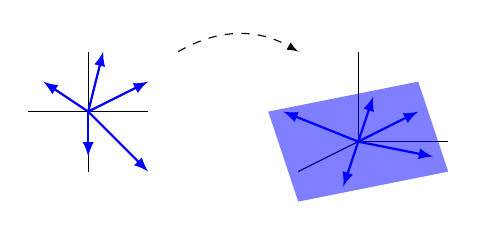
\begin{tikzpicture}[x=0.15in,y=0.15in]
  \begin{scope}[shift={(0,1)}]
    \draw (-2,0) -- (2,0);
    \draw (0,-2) -- (0,2);
    \draw[thick,-latex,blue] (0,0) -- (0.5,2);
    \draw[thick,-latex,blue] (0,0) -- (2,1);
    \draw[thick,-latex,blue] (0,0) -- (-1.5,1);
    \draw[thick,-latex,blue] (0,0) -- (0,-1.5);
    \draw[thick,-latex,blue] (0,0) -- (2,-2);
  \end{scope}
  \draw[dashed,-latex] (3,3) to [bend left=30] (7,3);
  \begin{scope}[shift={(9,0)}]
    \draw (0,0) -- (3,0);
    \draw (0,0) -- (0,3);
    \draw (0,0) -- (-2,-1);
    \draw[thick,-latex,blue] (0,0) -- (0.5,1.5);
    \draw[thick,-latex,blue] (0,0) -- (2,1);
    \draw[thick,-latex,blue] (0,0) -- (-2.5,1);
    \draw[thick,-latex,blue] (0,0) -- (-0.5,-1.5);
    \draw[thick,-latex,blue] (0,0) -- (2.5,-0.5);
    \fill[color=blue, opacity=0.5] (-2,-2) -- (3,-1) -- (2,2) -- (-3,1) -- (-2,-2);
  \end{scope}
\end{tikzpicture}
\end{center}
\end{definition}

\begin{activity}{5}
Let $T: \IR^2 \rightarrow \IR^3$ be given by
\[
  T\left(\begin{bmatrix}x \\ y \end{bmatrix} \right)
    =
  \begin{bmatrix} x \\ y \\ 0 \end{bmatrix}
    \hspace{3em}
    \text{with standard matrix }
  \begin{bmatrix} 1 & 0 \\ 0 & 1 \\ 0 & 0 \end{bmatrix}
\]
Which of these subspaces of \(\IR^3\) describes \(\Im T\),
the set of all vectors that are the result of using \(T\) to transform
\(\IR^2\) vectors?
\begin{multicols}{2}
\begin{enumerate}[a)]
\item \(\setBuilder{\begin{bmatrix}0 \\ 0\\ a\end{bmatrix}}{a\in\IR}\)
\item \(\setBuilder{\begin{bmatrix}a \\ b\\ 0\end{bmatrix}}{a,b\in\IR}\)
\item \(\setList{\begin{bmatrix}0\\0\\0\end{bmatrix}}\)
\item \(\IR^3=\setBuilder{\begin{bmatrix}x \\ y\\z\end{bmatrix}}{x,y,z\in\IR}\)
\end{enumerate}
\end{multicols}
\end{activity}

\begin{activity}{5}
Let $T: \IR^3 \rightarrow \IR^2$ be given by
\[
  T\left(\begin{bmatrix}x \\ y\\z \end{bmatrix} \right)
    =
  \begin{bmatrix} x \\ y \end{bmatrix}
    \hspace{3em}
    \text{with standard matrix }
  \begin{bmatrix} 1 & 0 & 0 \\ 0 & 1 & 0 \end{bmatrix}
\]
Which of these subspaces of \(\IR^2\) describes \(\Im T\),
the set of all vectors that are the result of using \(T\) to transform
\(\IR^3\) vectors?
\begin{enumerate}[a)]
\item \(\setBuilder{\begin{bmatrix}a \\ a\end{bmatrix}}{a\in\IR}\)
\item \(\setList{\begin{bmatrix}0\\0\end{bmatrix}}\)
\item \(\IR^2=\setBuilder{\begin{bmatrix}x \\ y\end{bmatrix}}{x,y\in\IR}\)
\end{enumerate}
\end{activity}


\begin{activity}{5}
Let $T: \IR^4 \rightarrow \IR^3$ be the linear transformation given by the
standard matrix
\[
  A
    =
  \begin{bmatrix} 3 & 4 & 7 & 1\\ -1 & 1 & 0 & 2 \\ 2 & 1 & 3 & -1 \end{bmatrix}
    =
  \begin{bmatrix}T(\vec e_1)&T(\vec e_2)&T(\vec e_3)&T(\vec e_4)\end{bmatrix}
.\]

Since \(T(\vec v)=T(x_1\vec e_1+x_2\vec e_2+x_3\vec e_3+x_4\vec e_4)\),
the set of vectors
\[
  \setList{
    \begin{bmatrix}3\\-1\\2\end{bmatrix},
    \begin{bmatrix}4\\1\\1\end{bmatrix},
    \begin{bmatrix}7\\0\\3\end{bmatrix},
    \begin{bmatrix}1\\2\\-1\end{bmatrix}
  }
\]
\begin{enumerate}[a)]
\item spans \(\Im T\)
\item is a linearly independent subset of \(\Im T\)
\item is a basis for \(\Im T\)
\end{enumerate}
\end{activity}


\begin{observation}
Let $T: \IR^4 \rightarrow \IR^3$ be the linear transformation given by the
standard matrix
\[
  A
    =
  \begin{bmatrix} 3 & 4 & 7 & 1\\ -1 & 1 & 0 & 2 \\ 2 & 1 & 3 & -1 \end{bmatrix}
.\]

Since the set
\(
  \setList{
    \begin{bmatrix}3\\-1\\2\end{bmatrix},
    \begin{bmatrix}4\\1\\1\end{bmatrix},
    \begin{bmatrix}7\\0\\3\end{bmatrix},
    \begin{bmatrix}1\\2\\-1\end{bmatrix}
  }
\)
spans \(\Im T\), we can obtain a basis for \(\Im T\) by finding
\(
  \RREF A
    =
  \begin{bmatrix} 1 & 0 & 1 & -1\\ 0 & 1 & 1 & 1 \\ 0 & 0 & 0 & 0 \end{bmatrix}
\)
and only using the vectors corresponding to pivot columns:
\[
  \setList{
    \begin{bmatrix}3\\-1\\2\end{bmatrix},
    \begin{bmatrix}4\\1\\1\end{bmatrix}
  }
\]
\end{observation}

\begin{fact}
Let  $T:\IR^n\to\IR^m$ be a linear transformation with standard matrix $A$.

\begin{itemize}
\item The kernel of \(T\) is the solution set of the homogeneous system given
by the augmented matrix $\begin{bmatrix}[c|c]A&\vec 0\end{bmatrix}$.
Use the coefficients of its free variables to get a basis for the kernel.
\item The image of \(T\) is the span of the columns of \(A\). Remove
the vectors creating non-pivot columns in \(\RREF A\) to get a basis
for the image.
\end{itemize}
\end{fact}


\begin{activity}{10}
Let $T: \IR^3 \rightarrow \IR^4$ be the linear transformation given by the
standard matrix
\[
  A
    =
  \begin{bmatrix} 1 & -3 & 2\\ 2 & -6 & 0 \\ 0 & 0 & 1 \\ -1 & 3 & 1 \end{bmatrix}
.\]

Find a basis for the kernel and a basis for the image of \(T\).
\end{activity}
\begin{definition}
Let $T: V \rightarrow W$ be a linear transformation.
$T$ is called \term{injective} or \term{one-to-one} if $T$ does not map two
distinct vectors to the same place.  More precisely, $T$ is injective if
$T(\vec{v}) \neq T(\vec{w})$ whenever $\vec{v} \neq \vec{w}$.

\begin{center}
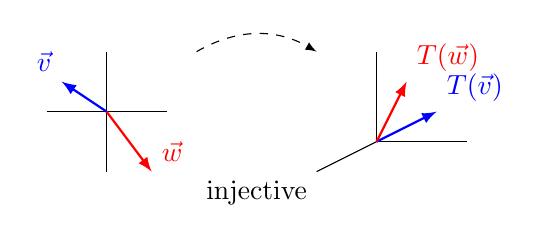
\begin{tikzpicture}[x=0.15in,y=0.15in]
  \begin{scope}[shift={(0,1)}]
    \draw (-2,0) -- (2,0);
    \draw (0,-2) -- (0,2);
    \draw[thick,-latex,blue] (0,0) -- (-1.5,1)
          node[anchor=south east] {\(\vec v\)};
    \draw[thick,-latex,red] (0,0) -- (1.5,-2)
          node[anchor=south west] {\(\vec w\)};
  \end{scope}
  \draw[dashed,-latex] (3,3) to [bend left=30] (7,3);
  \begin{scope}[shift={(9,0)}]
    \draw (0,0) -- (3,0);
    \draw (0,0) -- (0,3);
    \draw (0,0) -- (-2,-1);
    \draw[thick,-latex,blue] (0,0) -- (2,1)
          node[anchor=south west] {\(T(\vec v)\)};
    \draw[thick,-latex,red] (0,0) -- (1,2)
          node[anchor=south west] {\(T(\vec w)\)};
  \end{scope}
  \node[anchor=north] at (5,-1) {injective};
\end{tikzpicture}
\hspace{3em}
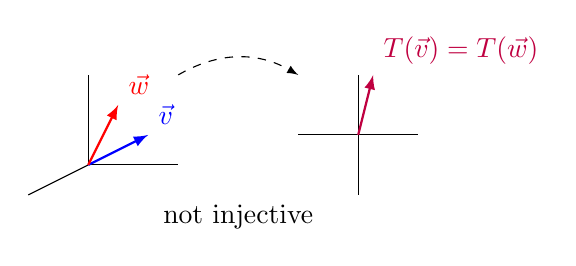
\begin{tikzpicture}[x=0.15in,y=0.15in]
  \begin{scope}[shift={(0,0)}]
    \draw (0,0) -- (3,0);
    \draw (0,0) -- (0,3);
    \draw (0,0) -- (-2,-1);
    \draw[thick,-latex,blue] (0,0) -- (2,1)
          node[anchor=south west] {\(\vec v\)};
    \draw[thick,-latex,red] (0,0) -- (1,2)
          node[anchor=south west] {\(\vec w\)};
  \end{scope}
  \draw[dashed,-latex] (3,3) to [bend left=30] (7,3);
  \begin{scope}[shift={(9,1)}]
    \draw (-2,0) -- (2,0);
    \draw (0,-2) -- (0,2);
    \draw[thick,-latex,purple] (0,0) -- (0.5,2)
          node[anchor=south west] {\(T(\vec v)=T(\vec w)\)};
  \end{scope}
  \node[anchor=north] at (5,-1) {not injective};
\end{tikzpicture}
\end{center}
\end{definition}

\begin{activity}{3}
Let $T: \IR^3 \rightarrow \IR^2$ be given by
\[
  T\left(\begin{bmatrix}x \\ y\\z \end{bmatrix} \right)
    =
  \begin{bmatrix} x \\ y \end{bmatrix}
    \hspace{3em}
    \text{with standard matrix }
  \begin{bmatrix} 1 & 0 & 0 \\ 0 & 1 & 0 \end{bmatrix}
\]
Is \(T\) injective?
\begin{enumerate}[a)]
\item Yes, because \(T(\vec v)=T(\vec w)\) whenever \(\vec v=\vec w\).
\item Yes, because \(T(\vec v)\not=T(\vec w)\) whenever \(\vec v\not=\vec w\).
\item No, because 
  \(
    T\left(\begin{bmatrix}0\\0\\1\end{bmatrix}\right)
      \not=
    T\left(\begin{bmatrix}0\\0\\2\end{bmatrix}\right)
  \)
\item No, because 
  \(
    T\left(\begin{bmatrix}0\\0\\1\end{bmatrix}\right)
      =
    T\left(\begin{bmatrix}0\\0\\2\end{bmatrix}\right)
  \)
\end{enumerate}
\end{activity}

\begin{activity}{2}
Let $T: \IR^2 \rightarrow \IR^3$ be given by
\[
  T\left(\begin{bmatrix}x \\ y \end{bmatrix} \right)
    =
  \begin{bmatrix} x \\ y \\ 0 \end{bmatrix}
    \hspace{3em}
    \text{with standard matrix }
  \begin{bmatrix} 1 & 0 \\ 0 & 1 \\ 0 & 0 \end{bmatrix}
\]
Is \(T\) injective?
\begin{enumerate}[a)]
\item Yes, because \(T(\vec v)=T(\vec w)\) whenever \(\vec v=\vec w\).
\item Yes, because \(T(\vec v)\not=T(\vec w)\) whenever \(\vec v\not=\vec w\).
\item No, because 
  \(
    T\left(\begin{bmatrix}1\\2\end{bmatrix}\right)
      \not=
    T\left(\begin{bmatrix}3\\4\end{bmatrix}\right)
  \)
\item No, because 
  \(
    T\left(\begin{bmatrix}1\\2\end{bmatrix}\right)
      =
    T\left(\begin{bmatrix}3\\4\end{bmatrix}\right)
  \)
\end{enumerate}
\end{activity}

\begin{definition}
Let $T: V \rightarrow W$ be a linear transformation.
$T$ is called \term{surjective} or \term{onto} if every element of $W$ is mapped to by an element of $V$.  More precisely, for every $\vec{w} \in W$, there is some $\vec{v} \in V$ with $T(\vec{v})=\vec{w}$.
\begin{center}
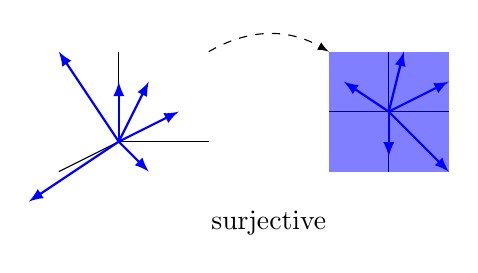
\begin{tikzpicture}[x=0.15in,y=0.15in]
  \begin{scope}[shift={(0,0)}]
    \draw (0,0) -- (3,0);
    \draw (0,0) -- (0,3);
    \draw (0,0) -- (-2,-1);
    \draw[thick,-latex,blue] (0,0) -- (2,1);
    \draw[thick,-latex,blue] (0,0) -- (1,2);
    \draw[thick,-latex,blue] (0,0) -- (0,2);
    \draw[thick,-latex,blue] (0,0) -- (1,-1);
    \draw[thick,-latex,blue] (0,0) -- (-2,3);
    \draw[thick,-latex,blue] (0,0) -- (-3,-2);
  \end{scope}
  \draw[dashed,-latex] (3,3) to [bend left=30] (7,3);
  \begin{scope}[shift={(9,1)}]
    \draw (-2,0) -- (2,0);
    \draw (0,-2) -- (0,2);
    \draw[thick,-latex,blue] (0,0) -- (0.5,2);
    \draw[thick,-latex,blue] (0,0) -- (2,1);
    \draw[thick,-latex,blue] (0,0) -- (-1.5,1);
    \draw[thick,-latex,blue] (0,0) -- (0,-1.5);
    \draw[thick,-latex,blue] (0,0) -- (2,-2);
    \fill[color=blue, opacity=0.5] (-2,-2) rectangle (2,2);
  \end{scope}
  \node[anchor=north] at (5,-2) {surjective};
\end{tikzpicture}
\hspace{3em}
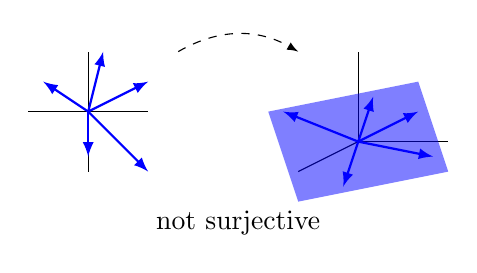
\begin{tikzpicture}[x=0.15in,y=0.15in]
  \begin{scope}[shift={(0,1)}]
    \draw (-2,0) -- (2,0);
    \draw (0,-2) -- (0,2);
    \draw[thick,-latex,blue] (0,0) -- (0.5,2);
    \draw[thick,-latex,blue] (0,0) -- (2,1);
    \draw[thick,-latex,blue] (0,0) -- (-1.5,1);
    \draw[thick,-latex,blue] (0,0) -- (0,-1.5);
    \draw[thick,-latex,blue] (0,0) -- (2,-2);
  \end{scope}
  \draw[dashed,-latex] (3,3) to [bend left=30] (7,3);
  \begin{scope}[shift={(9,0)}]
    \draw (0,0) -- (3,0);
    \draw (0,0) -- (0,3);
    \draw (0,0) -- (-2,-1);
    \draw[thick,-latex,blue] (0,0) -- (0.5,1.5);
    \draw[thick,-latex,blue] (0,0) -- (2,1);
    \draw[thick,-latex,blue] (0,0) -- (-2.5,1);
    \draw[thick,-latex,blue] (0,0) -- (-0.5,-1.5);
    \draw[thick,-latex,blue] (0,0) -- (2.5,-0.5);
    \fill[color=blue, opacity=0.5] (-2,-2) -- (3,-1) -- (2,2) -- (-3,1) -- (-2,-2);
  \end{scope}
  \node[anchor=north] at (5,-2) {not surjective};
\end{tikzpicture}
\end{center}
\end{definition}

\begin{activity}{3}
Let $T: \IR^2 \rightarrow \IR^3$ be given by
\[
  T\left(\begin{bmatrix}x \\ y \end{bmatrix} \right)
    =
  \begin{bmatrix} x \\ y \\ 0 \end{bmatrix}
    \hspace{3em}
    \text{with standard matrix }
  \begin{bmatrix} 1 & 0 \\ 0 & 1 \\ 0 & 0 \end{bmatrix}
\]
Is \(T\) surjective?
\begin{enumerate}[a)]
\item Yes, because for every \(\vec w=\begin{bmatrix}x\\y\\z\end{bmatrix}\in\IR^3\),
there exists \(\vec v=\begin{bmatrix}x\\y\end{bmatrix}\in\IR^2\) such that
\(T(\vec v)=\vec w\).
\item No, because 
  \(
    T\left(\begin{bmatrix}x\\y\end{bmatrix}\right)
  \)
can never equal
  \(
  \begin{bmatrix} 1 \\ 1 \\ 1 \end{bmatrix}
  \).
\item No, because 
  \(
    T\left(\begin{bmatrix}x\\y\end{bmatrix}\right)
  \)
can never equal
  \(
  \begin{bmatrix} 0 \\ 0 \\ 0 \end{bmatrix}
  \).
\end{enumerate}
\end{activity}

\begin{activity}{2}
Let $T: \IR^3 \rightarrow \IR^2$ be given by
\[
  T\left(\begin{bmatrix}x \\ y\\z \end{bmatrix} \right)
    =
  \begin{bmatrix} x \\ y \end{bmatrix}
    \hspace{3em}
    \text{with standard matrix }
  \begin{bmatrix} 1 & 0 & 0 \\ 0 & 1 & 0 \end{bmatrix}
\]
Is \(T\) surjective?
\begin{enumerate}[a)]
\item Yes, because for every \(\vec w=\begin{bmatrix}x\\y\end{bmatrix}\in\IR^2\),
there exists \(\vec v=\begin{bmatrix}x\\y\\42\end{bmatrix}\in\IR^3\) such that
\(T(\vec v)=\vec w\).
\item Yes, because for every \(\vec w=\begin{bmatrix}x\\y\end{bmatrix}\in\IR^2\),
there exists \(\vec v=\begin{bmatrix}0\\0\\z\end{bmatrix}\in\IR^3\) such that
\(T(\vec v)=\vec w\).
\item No, because 
  \(
    T\left(\begin{bmatrix}x\\y\\z\end{bmatrix}\right)
  \)
can never equal
  \(
  \begin{bmatrix} 3\\-2 \end{bmatrix}
  \).
\end{enumerate}
\end{activity}

\begin{observation}
As we will see, it's no coincidence that the \(\RREF\) of the
injective map's standard matrix
\[
  \begin{bmatrix} 1 & 0 \\ 0 & 1 \\ 0 & 0 \end{bmatrix}
\]
has all pivot columns. Similarly, the \(\RREF\) of the surjective map's
standard matrix
\[
  \begin{bmatrix} 1 & 0 & 0 \\ 0 & 1 & 0 \end{bmatrix}
\]
has a pivot in each row.
\end{observation}




\begin{observation}
Let \(T: V \rightarrow W\).  We have previously defined the following
terms.
\begin{itemize}
\item The \term{kernel} of \(T\) is the set of all vectors in \(V\) that are mapped to $\vec{z}\in W$.  It is a subspace of \(V\).
\item The \term{image} of \(T\) is the set of all vectors in \(W\) that are mapped to by something in \(V\).  It is a subspace of \(W\).
\item  \(T\) is called \term{injective} or \term{one-to-one} if \(T\) always maps  distinct vectors to different places.
\item \(T\) is called \term{surjective} or \term{onto} if every element of \(W\) is mapped to by some element of \(V\).
\end{itemize}
\end{observation}

\begin{activity}{5}
Let \(T: V \rightarrow W\) be a linear transformation where
\(\ker T\) contains multiple vectors. What can you conclude?
\begin{enumerate}[(a)]
\item \(T\) is injective
\item \(T\) is not injective
\item \(T\) is surjective
\item \(T\) is not surjective
\end{enumerate}
\end{activity}

\begin{fact}
A linear transformation $T$ is injective \textbf{if and only if} $\ker T = \{\vec{0}\}$. Put another way, an injective linear transformation may be
recognized by its \term{trivial} kernel.

\begin{center}
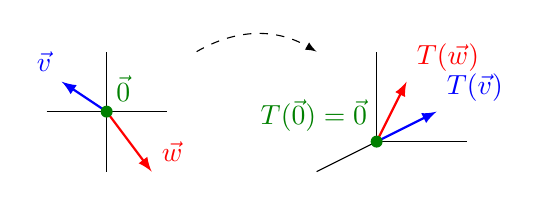
\begin{tikzpicture}[x=0.15in,y=0.15in]
  \begin{scope}[shift={(0,1)}]
    \draw (-2,0) -- (2,0);
    \draw (0,-2) -- (0,2);
    \draw[thick,-latex,blue] (0,0) -- (-1.5,1)
          node[anchor=south east] {\(\vec v\)};
    \draw[thick,-latex,red] (0,0) -- (1.5,-2)
          node[anchor=south west] {\(\vec w\)};
    \fill[green!50!black] (0,0) circle (0.2)
          node[anchor=south west] {\(\vec{0}\)};
  \end{scope}
  \draw[dashed,-latex] (3,3) to [bend left=30] (7,3);
  \begin{scope}[shift={(9,0)}]
    \draw (0,0) -- (3,0);
    \draw (0,0) -- (0,3);
    \draw (0,0) -- (-2,-1);
    \draw[thick,-latex,blue] (0,0) -- (2,1)
          node[anchor=south west] {\(T(\vec v)\)};
    \draw[thick,-latex,red] (0,0) -- (1,2)
          node[anchor=south west] {\(T(\vec w)\)};
    \fill[green!50!black] (0,0) circle (0.2)
          node[anchor=south east] {\(T(\vec{0})=\vec{0}\)};
  \end{scope}
\end{tikzpicture}
\end{center}
\end{fact}

\begin{activity}{5}
Let $T: V \rightarrow \IR^5$ be a linear transformation where
$\Im T$ is spanned by four vectors.
What can you conclude?
\begin{enumerate}[(a)]
\item \(T\) is injective
\item \(T\) is not injective
\item \(T\) is surjective
\item \(T\) is not surjective
\end{enumerate}
\end{activity}

\begin{fact}
A linear transformation $T:V \rightarrow W$ is surjective \textbf{if and only if} $\Im T = W$. Put another way, a surjective linear transformation may be
recognized by its identical codomain and image.
\begin{center}
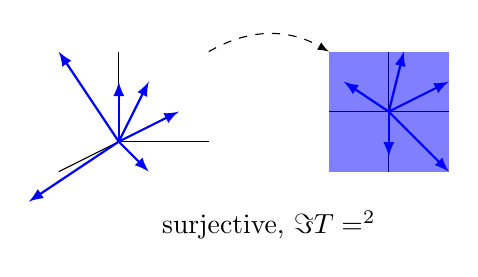
\begin{tikzpicture}[x=0.15in,y=0.15in]
  \begin{scope}[shift={(0,0)}]
    \draw (0,0) -- (3,0);
    \draw (0,0) -- (0,3);
    \draw (0,0) -- (-2,-1);
    \draw[thick,-latex,blue] (0,0) -- (2,1);
    \draw[thick,-latex,blue] (0,0) -- (1,2);
    \draw[thick,-latex,blue] (0,0) -- (0,2);
    \draw[thick,-latex,blue] (0,0) -- (1,-1);
    \draw[thick,-latex,blue] (0,0) -- (-2,3);
    \draw[thick,-latex,blue] (0,0) -- (-3,-2);
  \end{scope}
  \draw[dashed,-latex] (3,3) to [bend left=30] (7,3);
  \begin{scope}[shift={(9,1)}]
    \draw (-2,0) -- (2,0);
    \draw (0,-2) -- (0,2);
    \draw[thick,-latex,blue] (0,0) -- (0.5,2);
    \draw[thick,-latex,blue] (0,0) -- (2,1);
    \draw[thick,-latex,blue] (0,0) -- (-1.5,1);
    \draw[thick,-latex,blue] (0,0) -- (0,-1.5);
    \draw[thick,-latex,blue] (0,0) -- (2,-2);
    \fill[color=blue, opacity=0.5] (-2,-2) rectangle (2,2);
  \end{scope}
  \node[anchor=north] at (5,-2) {surjective, \(\Im T=\IR^2\)};
\end{tikzpicture}
\hspace{3em}
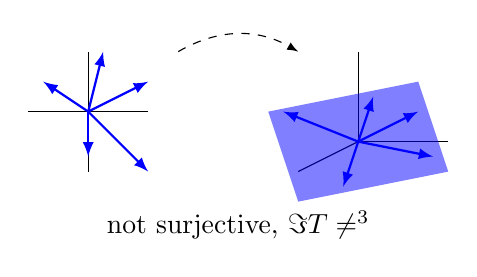
\begin{tikzpicture}[x=0.15in,y=0.15in]
  \begin{scope}[shift={(0,1)}]
    \draw (-2,0) -- (2,0);
    \draw (0,-2) -- (0,2);
    \draw[thick,-latex,blue] (0,0) -- (0.5,2);
    \draw[thick,-latex,blue] (0,0) -- (2,1);
    \draw[thick,-latex,blue] (0,0) -- (-1.5,1);
    \draw[thick,-latex,blue] (0,0) -- (0,-1.5);
    \draw[thick,-latex,blue] (0,0) -- (2,-2);
  \end{scope}
  \draw[dashed,-latex] (3,3) to [bend left=30] (7,3);
  \begin{scope}[shift={(9,0)}]
    \draw (0,0) -- (3,0);
    \draw (0,0) -- (0,3);
    \draw (0,0) -- (-2,-1);
    \draw[thick,-latex,blue] (0,0) -- (0.5,1.5);
    \draw[thick,-latex,blue] (0,0) -- (2,1);
    \draw[thick,-latex,blue] (0,0) -- (-2.5,1);
    \draw[thick,-latex,blue] (0,0) -- (-0.5,-1.5);
    \draw[thick,-latex,blue] (0,0) -- (2.5,-0.5);
    \fill[color=blue, opacity=0.5] (-2,-2) -- (3,-1) -- (2,2) -- (-3,1) -- (-2,-2);
  \end{scope}
  \node[anchor=north] at (5,-2) {not surjective, \(\Im T\not=\IR^3\)};
\end{tikzpicture}
\end{center}
\end{fact}

\begin{activity}{15}
Let $T: \IR^n \rightarrow \IR^m$ be a linear map with standard matrix $A$.
Sort the following claims into two groups of \textit{equivalent} statements:
one group that means \(T\) is \textbf{injective}, and one group that means
\(T\) is \textbf{surjective}.
\begin{multicols}{2}
\begin{enumerate}[(a)]
\item The kernel of \(T\) is trivial, i.e. \(\ker T=\{\vec 0\}\).
\item The columns of $A$ span $\IR^m$.
\item The columns of $A$ are linearly independent.
\item Every column of $\RREF(A)$ has a pivot.
\item Every row of $\RREF(A)$ has a pivot.
\item The image of \(T\) equals its codomain, i.e. \(\Im T=\IR^m\).
\item The system of linear equations given by the augmented matrix $\begin{bmatrix}[c|c]A & \vec{b} \end{bmatrix}$ has a solution for all $\vec{b} \in \IR^m$.
\item The system of linear equations given by the augmented matrix $\begin{bmatrix}[c|c] A & \vec{0} \end{bmatrix}$ has exactly one solution.
\end{enumerate}
\end{multicols}
\begin{instructorNote}
  This activity may be ran as a card sort.
\end{instructorNote}
\end{activity}

\begin{observation}
  The easiest way to show that the linear map with standard matrix \(A\)
  is injective is to show that \(\RREF(A)\) has a pivot in each column.

  \vspace{1em}

  The easiest way to show that the linear map with standard matrix \(A\)
  is surjective is to show that \(\RREF(A)\) has a pivot in each row.
\end{observation}

\begin{activity}{3}
  What can you conclude about the linear map 
  \(T:\IR^2\to\IR^3\) with standard matrix 
  \(\begin{bmatrix} a & b \\ c & d \\ e & f \end{bmatrix}\)?
  \begin{enumerate}[a)]
    \item Its standard matrix has more columns than rows, so \(T\) is not
    injective.
    \item Its standard matrix has more columns than rows, so \(T\) is
    injective.
    \item Its standard matrix has more rows than columns, so \(T\) is not
    surjective.
    \item Its standard matrix has more rows than columns, so \(T\) is
    surjective.
  \end{enumerate}
\end{activity}

\begin{activity}{2}
  What can you conclude about the linear map \(T:\IR^3\to\IR^2\) with standard matrix 
  \(\begin{bmatrix} a & b & c \\ d & e & f \end{bmatrix}\)?
  \begin{enumerate}[a)]
    \item Its standard matrix has more columns than rows, so \(T\) is not
    injective.
    \item Its standard matrix has more columns than rows, so \(T\) is
    injective.
    \item Its standard matrix has more rows than columns, so \(T\) is not
    surjective.
    \item Its standard matrix has more rows than columns, so \(T\) is
    surjective.
  \end{enumerate}
\end{activity}

\begin{fact}
  The following are true for any linear map \(T:V\to W\):
  \begin{itemize}
    \item If \(\dim(V)>\dim(W)\), then \(T\) is not injective.
    \item If \(\dim(V)<\dim(W)\), then \(T\) is not surjective.
  \end{itemize}
  Basically, a linear transformation cannot reduce dimension without collapsing
  vectors into each other, and a linear transformation cannot
  increase dimension from its domain to its image.
  \begin{center}
    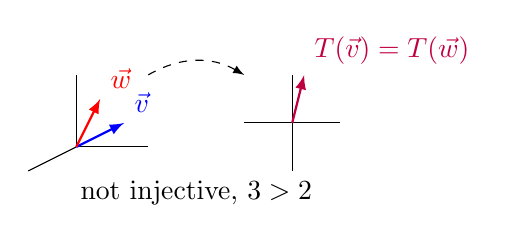
\begin{tikzpicture}[x=0.12in,y=0.12in]
      \begin{scope}[shift={(0,0)}]
        \draw (0,0) -- (3,0);
        \draw (0,0) -- (0,3);
        \draw (0,0) -- (-2,-1);
        \draw[thick,-latex,blue] (0,0) -- (2,1)
              node[anchor=south west] {\(\vec v\)};
        \draw[thick,-latex,red] (0,0) -- (1,2)
              node[anchor=south west] {\(\vec w\)};
      \end{scope}
      \draw[dashed,-latex] (3,3) to [bend left=30] (7,3);
      \begin{scope}[shift={(9,1)}]
        \draw (-2,0) -- (2,0);
        \draw (0,-2) -- (0,2);
        \draw[thick,-latex,purple] (0,0) -- (0.5,2)
              node[anchor=south west] {\(T(\vec v)=T(\vec w)\)};
      \end{scope}
      \node[anchor=north] at (5,-1) {not injective, \(3>2\)};
    \end{tikzpicture}
    \hspace{3em}
    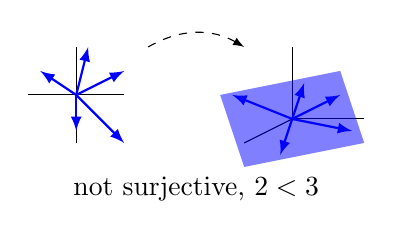
\begin{tikzpicture}[x=0.12in,y=0.12in]
      \begin{scope}[shift={(0,1)}]
        \draw (-2,0) -- (2,0);
        \draw (0,-2) -- (0,2);
        \draw[thick,-latex,blue] (0,0) -- (0.5,2);
        \draw[thick,-latex,blue] (0,0) -- (2,1);
        \draw[thick,-latex,blue] (0,0) -- (-1.5,1);
        \draw[thick,-latex,blue] (0,0) -- (0,-1.5);
        \draw[thick,-latex,blue] (0,0) -- (2,-2);
      \end{scope}
      \draw[dashed,-latex] (3,3) to [bend left=30] (7,3);
      \begin{scope}[shift={(9,0)}]
        \draw (0,0) -- (3,0);
        \draw (0,0) -- (0,3);
        \draw (0,0) -- (-2,-1);
        \draw[thick,-latex,blue] (0,0) -- (0.5,1.5);
        \draw[thick,-latex,blue] (0,0) -- (2,1);
        \draw[thick,-latex,blue] (0,0) -- (-2.5,1);
        \draw[thick,-latex,blue] (0,0) -- (-0.5,-1.5);
        \draw[thick,-latex,blue] (0,0) -- (2.5,-0.5);
        \fill[color=blue, opacity=0.5] (-2,-2) -- (3,-1) -- (2,2) -- (-3,1) -- (-2,-2);
      \end{scope}
      \node[anchor=north] at (5,-2) {not surjective, \(2<3\)};
    \end{tikzpicture}
    \end{center}
  But dimension arguments \textbf{cannot} be used to prove a map \textbf{is}
  injective or surjective.
\end{fact}


\begin{activity}{5}
Suppose \(T: \IR^n \rightarrow \IR^4\) with standard matrix 
\(A=\begin{bmatrix}
  a_{11}&a_{12}&\cdots&a_{1n}\\
  a_{21}&a_{22}&\cdots&a_{2n}\\
  a_{31}&a_{32}&\cdots&a_{3n}\\
  a_{41}&a_{42}&\cdots&a_{4n}\\
\end{bmatrix}\) is both 
injective and surjective (we call such maps \term{bijective}).
\begin{subactivity}
How many pivot rows must \(\RREF A\) have?
\end{subactivity}
\begin{subactivity}
 How many pivot columns must \(\RREF A\) have?
\end{subactivity}
\begin{subactivity}
What is \(\RREF A\)?
\end{subactivity}
\end{activity}


\begin{activity}{5}
Let $T: \IR^n \rightarrow \IR^n$ be a bijective linear map with
standard matrix $A$. Label each of the following as true or false.
\begin{enumerate}[(a)]
\item $\RREF(A)$ is the identity matrix.
\item The columns of $A$ form a basis for $\IR^n$
\item The system of linear equations given by the augmented matrix $\begin{bmatrix}[c|c] A & \vec{b} \end{bmatrix}$ has exactly one solution
for each \(\vect b \in \IR^n\).
\end{enumerate}
\end{activity}

\begin{observation}
  The easiest way to show that the linear map with standard matrix \(A\)
  is bijective is to show that \(\RREF(A)\) is the identity matrix.
\end{observation}

\begin{activity}{3}
Let $T: \IR^3 \rightarrow \IR^3$ be given by the standard matrix $$A=\begin{bmatrix} 2&1&-1 \\ 4&1&1 \\ 6&2&1\end{bmatrix}.$$ Which of the following must be true?
\begin{enumerate}[(a)]
\item $T$ is neither injective nor surjective
\item $T$ is injective but not surjective
\item $T$ is surjective but not injective
\item $T$ is bijective.
\end{enumerate}
\end{activity}

\begin{activity}{3}
Let $T: \IR^3 \rightarrow \IR^3$ be given by $$T\left(\begin{bmatrix} x \\ y  \\ z \end{bmatrix} \right) = \begin{bmatrix} 2x+y-z \\ 4x+y+z \\ 6x+2y\end{bmatrix}.$$   Which of the following must be true?
\begin{enumerate}[(a)]
\item $T$ is neither injective nor surjective
\item $T$ is injective but not surjective
\item $T$ is surjective but not injective
\item $T$ is bijective.
\end{enumerate}
\end{activity}

\begin{activity}{3}
Let $T: \IR^2 \rightarrow \IR^3$ be given by $$T\left(\begin{bmatrix} x \\ y \end{bmatrix} \right) = \begin{bmatrix} 2x+3y \\ x-y \\ x+3y\end{bmatrix}.$$  Which of the following must be true?
\begin{enumerate}[(a)]
\item $T$ is neither injective nor surjective
\item $T$ is injective but not surjective
\item $T$ is surjective but not injective
\item $T$ is bijective.
\end{enumerate}
\end{activity}

\begin{activity}{3}
Let $T: \IR^3 \rightarrow \IR^2$ be given by $$T\left(\begin{bmatrix} x \\ y  \\ z \end{bmatrix} \right) = \begin{bmatrix} 2x+y-z \\ 4x+y+z\end{bmatrix}.$$  Which of the following must be true?
\begin{enumerate}[(a)]
\item $T$ is neither injective nor surjective
\item $T$ is injective but not surjective
\item $T$ is surjective but not injective
\item $T$ is bijective.
\end{enumerate}
\end{activity}

